
\begin{frame}
\frametitle{\secname}
\begin{timeline}{1965}{2018}{2cm}{2.5cm}{7cm}{6cm}
	\entry{1968}{Theorie: Elektroschwache Wechselwirkung}
	\pause\entry{1973}{Indirekter Nachweise neutraler Ströme}
	\pause\entry{1983}{Direkte Entdeckung}
	\pause\entry{1989}{Präzisionsmessungen am LEP}
	\pause\entry{2012}{Nachweis des Higg-Bosons am CERN}
	\onslide<1->
\end{timeline}

\only<1> {
	\begin{textblock*}{5cm}(7cm,3cm) % {block width} (coords)
	\begin{figure}
		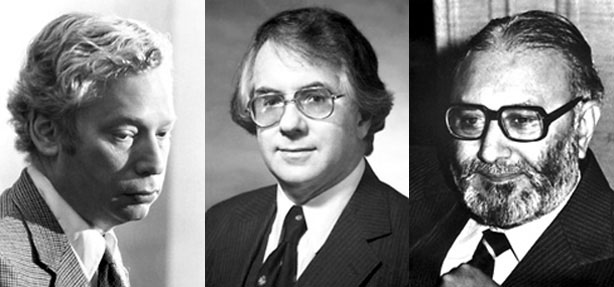
\includegraphics[width=4cm]{img/weinberg_glasgow_salam}
		\caption*{Steven Weinberg, Sheldon Glashow und Abdus Salam \cite{GSW}}
	\end{figure}
\end{textblock*}
}
\only<2> {
	\begin{textblock*}{3.6cm}(4.5cm,3.5cm) % {block width} (coords)
	\begin{figure}
		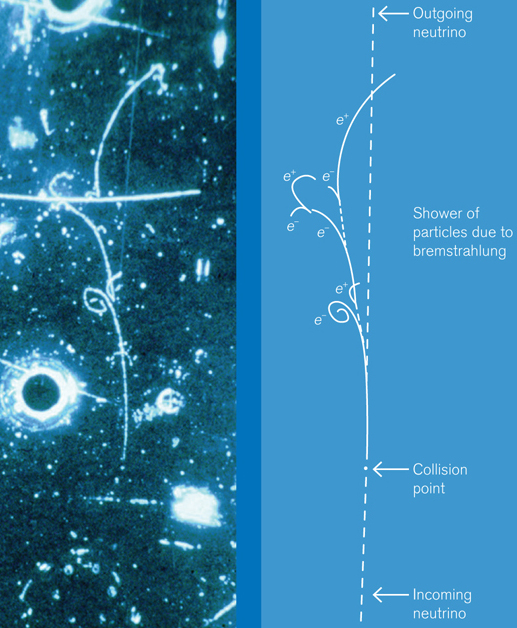
\includegraphics[width=3.6cm,angle=-90]{img/neutralerstrom}
		\caption*{$\bar{\nu}_\mu + e^- \rightarrow \bar{\nu}_\mu + e^-$ \cite{HASERT1973121}}
	\end{figure}
\end{textblock*}
}
\note[item] {Vereinheitlichung von elektr. + schwache WW. Kräfteaustausch durch Photon,$W^\pm$, $Z^0$}
\note[item]{1979 Nobelpreis für GWS}
\note[item]{Neutrale Ströme von links nach rechts Antineutrinostrahl in Blasenkammer. Photon nur bei elektr. Prozessen.(=> neutraler Strom, Z) Anhand von Winkel und 1/3 Energie des $e^-$ folgt Wechselwirkung durch neutrale Ströme. 700000 - Bilder überprüft. Spiral/Bremsstrahlung.}
\note[item]{CERN}%TODO
\note[item]{Large Electron Positron Ring (CERN) Präzessionsmessungen weiter Bestätigtbis 2000}
\note[item]{2013 Francois Englert und Peter Higgs Nobelpreis}
\end{frame}
